\chapter{Project Architecture}
 \begin{sidewaysfigure}[h!tb]
    \centering
    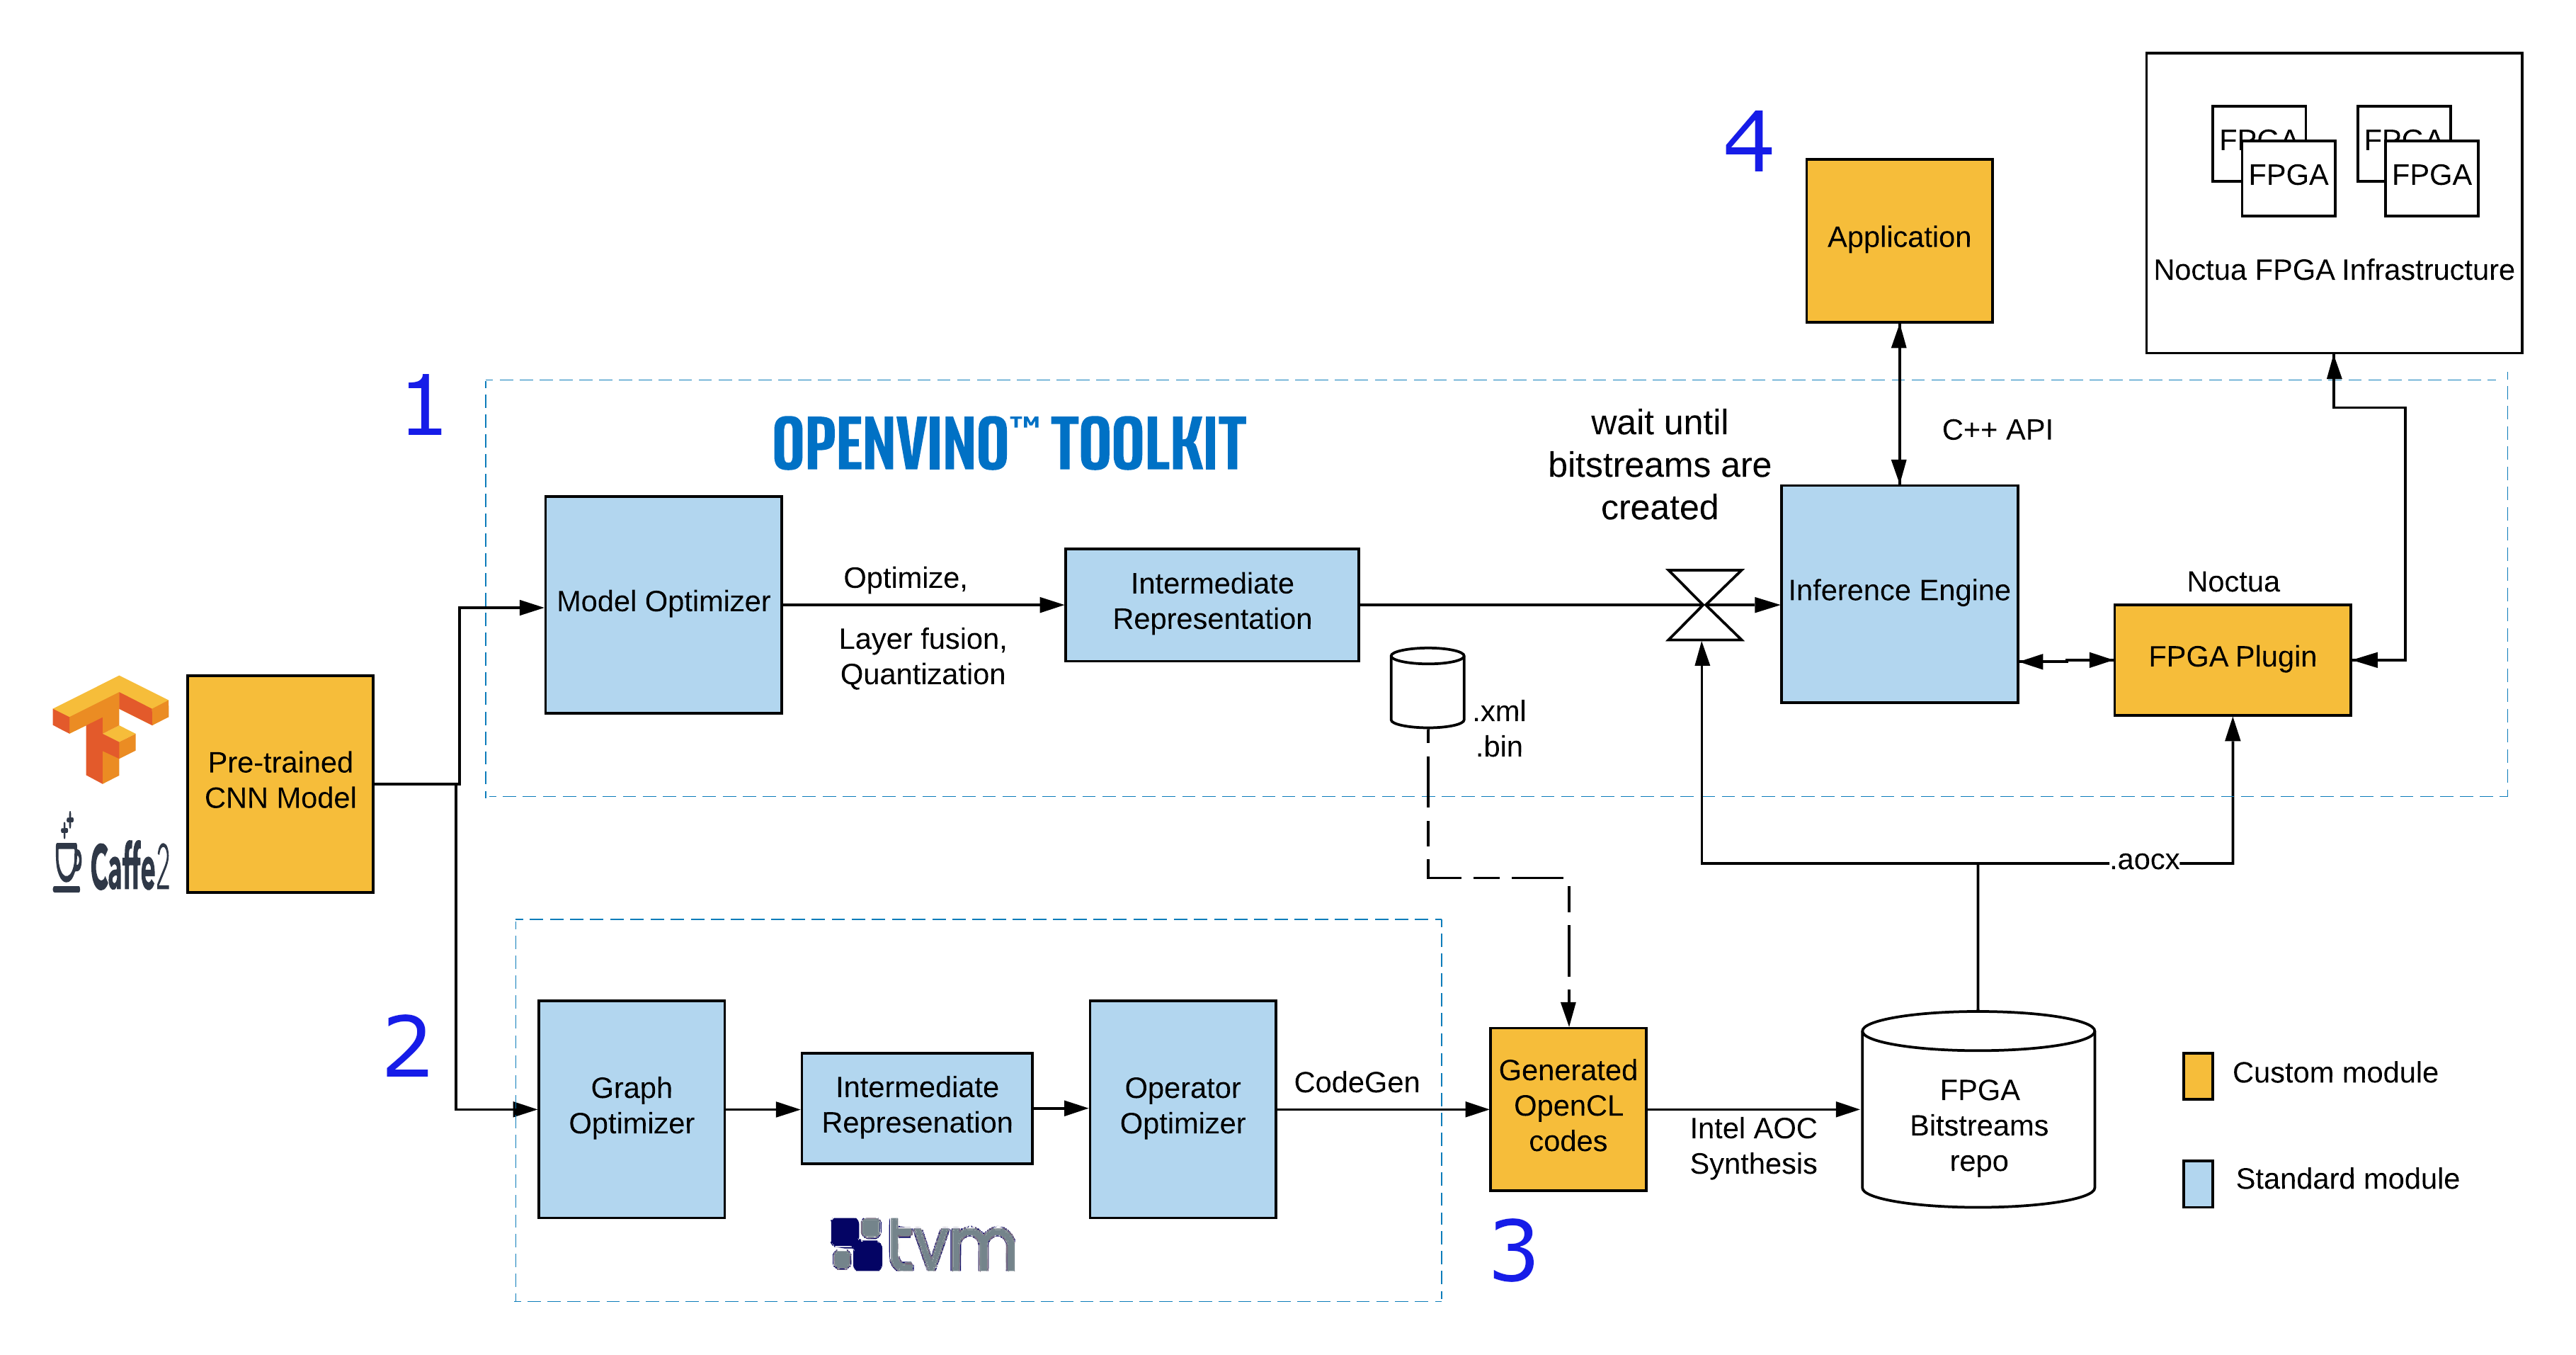
\includegraphics[scale=1,width=\textwidth]{img/CustoNN2_Workflow_New.png}
    \caption{CustoNN2 Project Workflow}
    \label{fig:custonn2_workflow}
\end{sidewaysfigure}
Figure \ref{fig:custonn2_workflow} describes the workflow of the project group. As mentioned in Chapter \ref{chp:Toolkits}, we used two toolkits in our project. The workflow has four following important steps(numbered in Figure \ref{fig:custonn2_workflow}):
\subsection*{Step 1: Generating OpenVINO IR}
First starting with OpenVINO, we feed the downloaded pre-trained CNN model to the OpenVINO Model Optimizer. In Model Optimizer, the trained model in the form of \textit{protobuf} file undergoes optimizations and and get converted to a file format which can be read,loaded and inferred by OpenVINO Inference Engine. The output of Model Optimizer is an Intermediate Representation (IR) consisting of an XML file and a binary(.bin) file. The XML file contains the description of the CNN model topology and the .bin file contains the biases and weights binary data. 
 
\subsection*{Step 2: Generating OpenCL Kernels}

We feed the downloaded pre-trained frozen CNN model to the NNVM compiler. The compiler frontend parses the model generating  NNVM expression (sym) and parameters (params) from the model. We set the optimization level and based on this level graph optimization techniques such as Operator Fusion and DataLayout Formatting are performed. The output is an Intermediate Representation (IR) which contains two files. The first is a JSON file that contains the optimized computational graph and the second file is a PARAM file that contains the quantized weight of the CNN model. This high-level IR and optimized computational graph are sent to lowering function with a TVMRegister API call which generates lower-level IR and graph. This code is then passed to the CodeGen module of the TVM toolkit and based on the target hradware it generates the required OpenCL kernel codes. The generated OpenCL kernel codes can be specific to a particular topology or it can be layer-specific which can be used in multiple topologies.

Step 1 and 2 are independent of each other and can be executed parallely.
 
These generated OpenCL kernel code needs to be customized to be compatible with OpenVINO FPGA plugin. After customization these kernel code are then synthesized for Stratix 10 FPGAs in the Noctua cluster and we create a repository of these bitstreams. We use TVM toolkit solely as a code generator for OpenCL kernel codes.

\subsection*{Step 3: Integrating toolkits and bitstream synthesis}
By default, the toolkits cannot work together and hence we need explicit integration in our workflow. The dotted arrow line in the Figure \ref{fig:custonn2_workflow} shows the integration point.
The OpenCL kernels generated by TVM are customized to be compatible with OpenVINO FPGA plugin. Here we manually change the OpenCL kernel names according to the OpenVINO IR layer names. Along with the layer names, for integration we had to change the layout of the some kernels (for ex: Concat kernels in GoogLeNet) from NHWC to NCHW. Once all the kernels are tested for correctness, we divide the OpenCL kernel file into multiple kernel files accordig to the scaling strategy. After customization these kernel code are then synthesized for Stratix 10 FPGAs in the Noctua cluster and we create a repository of these bitstreams. 
  
\subsection*{Step 4: Inference}
We have to wait till Step 3 is completed and all the bitstreams are synthesised without any errors.

The inference is done using a C++ application which uses OpenVINO Inference Engine and FPGA plugin  for the image classification in the Noctua cluster. The application is executed on multiple nodes of the Noctua FPGA nodes simultaneously according to the scaling strategy. The synchronisation between multiple application instances are done with the help of MPI barrier.

First, according to the scaling strategy the FPGA plugin will flash the appropriate bitstreams on the devices at each Noctua FPGA node. Once all the bitstreams are flashed on the FPGAs, the plugin will parse the Intermediate Representation (IR) information and start the inference on the FPGA by launching the OpenCL kernels.
After the execution of whole CNN topology, the instance of the application running on the last FPGA node will give the inference results with the TopN image classification with its Softmax values.



\begin{figure}[!htbp]
   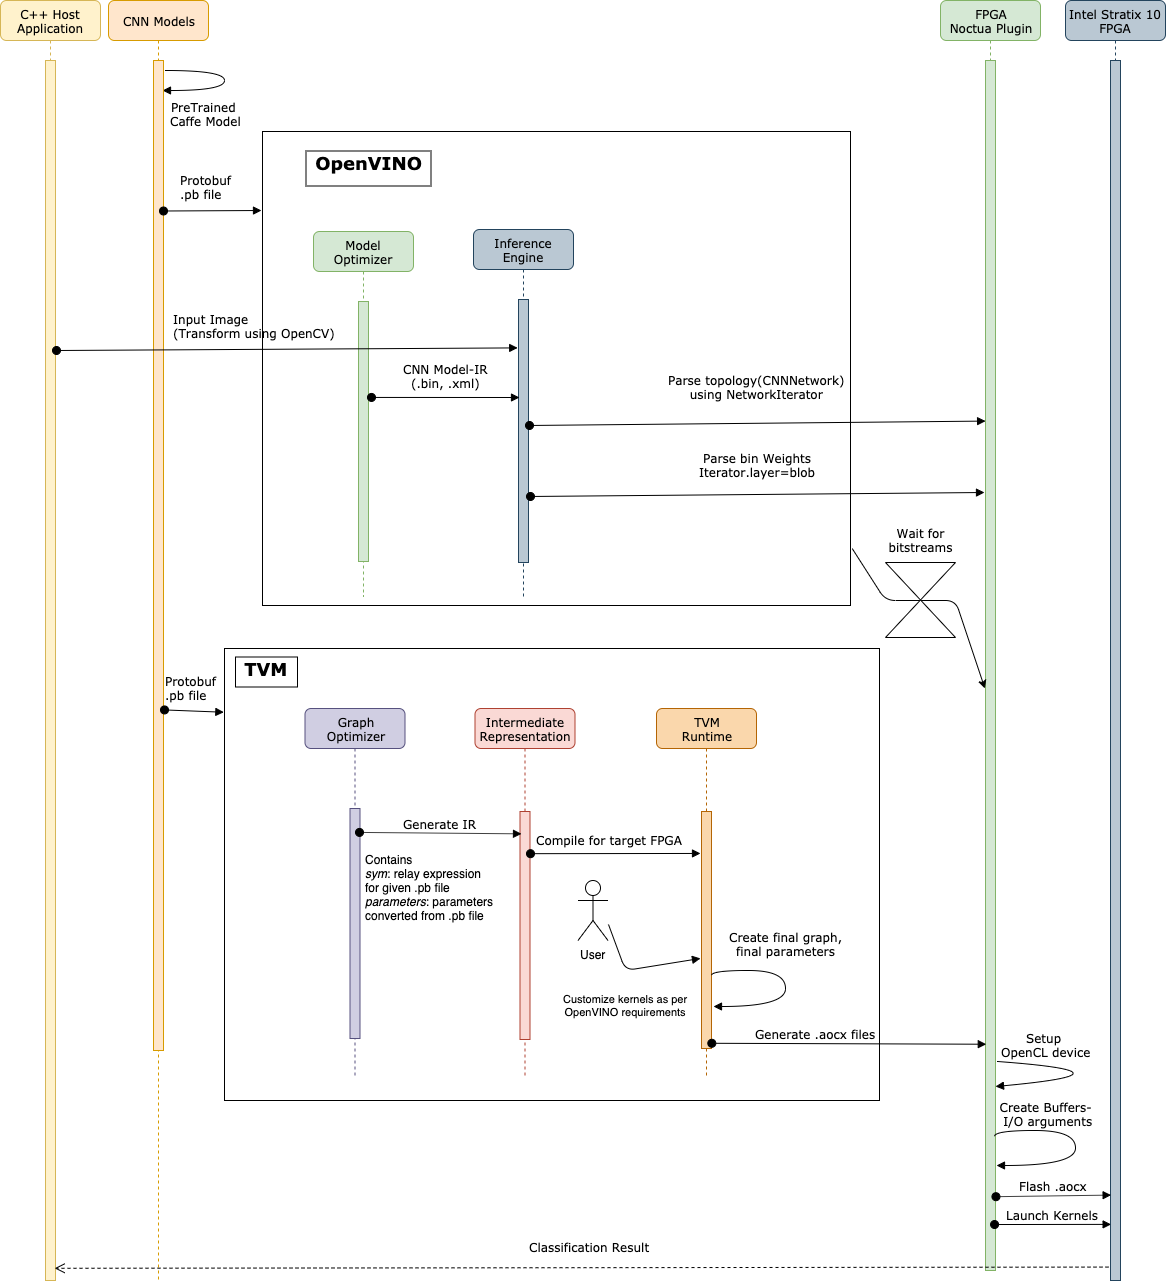
\includegraphics[width=\textwidth,height=\textheight]{img/udd.png}
   \caption{Sequence Diagram of the Project Workflow}
\end{figure}
